% =====================================================================
\section{Directional Derivatives}\label{ch:dirder}
% =====================================================================

\subsection{Motivation: slopes in an arbitrary direction}

Recall from Chapter~\ref{ch:prelim} that, for $z=f(x,y)$,
\[
  f_x(x_0,y_0)=\lim_{h\to0}\frac{f(x_0+h,y_0)-f(x_0,y_0)}{h},\qquad
  f_y(x_0,y_0)=\lim_{h\to0}\frac{f(x_0,y_0+h)-f(x_0,y_0)}{h}
\]
represent the rates of change of $z$ in the $x$- and $y$-directions, that is,
in the directions of the unit vectors $\vi$ and $\vj$ (Slides, \emph{Partial
Derivatives}).

Imagine standing on the hill $z=f(x,y)$ at the point above $(x_0,y_0)$. Walking
due east (direction $\vi$) the ground rises at rate $f_x$; walking due north
(direction $\vj$) it rises at rate $f_y$. But you can walk in \emph{any}
direction, say north-east, or towards a landmark $Q$. How steep is the hill in
that direction? The \emph{directional derivative} answers this question.

Geometrically, fix a unit vector $\vu=\ip{a,b}$. The vertical plane through
$P(x_0,y_0,f(x_0,y_0))$ in the direction of $\vu$ cuts the surface in a curve
$C$. The directional derivative $\Du f(x_0,y_0)$ is the slope of the tangent
line to $C$ at $P$ (Figure~\ref{fig:surface-slice}).

\begin{figure}[H]
  \centering
  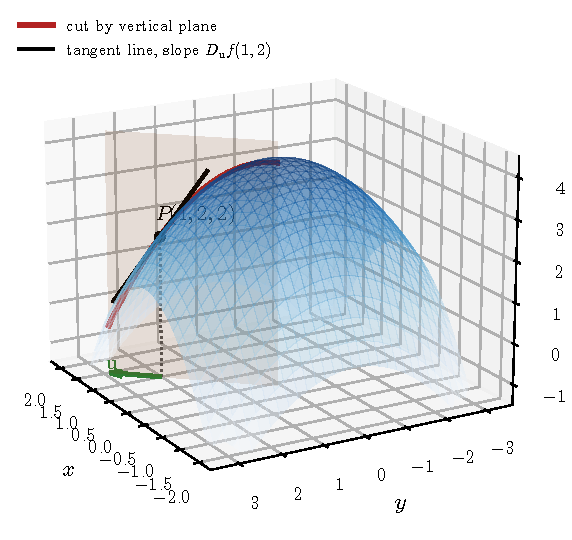
\includegraphics[width=0.66\linewidth]{surface_slice}
  \caption{The surface $z=4-x^2-\tfrac14y^2$ of Slides, Example~6.1, cut by the
  vertical plane through $(1,2)$ in the direction
  $\vu=\ip{\cos\frac\pi3,\sin\frac\pi3}$. The slope of the black tangent line is
  $\Du f(1,2)=-1-\frac{\sqrt3}{2}\approx-1.87$: walking in direction $\vu$ you go
  \emph{downhill}.}
  \label{fig:surface-slice}
\end{figure}

\subsection{Definition}

If we move from $(x_0,y_0)$ a distance $h$ in the direction of the \emph{unit}
vector $\vu=\ip{a,b}$, we arrive at $(x_0+ha,\,y_0+hb)$. Comparing the change
in $f$ with the distance $h$ travelled gives the following definition.

\begin{definition}[Directional derivative; Slides]\label{def:Du}
The \emph{directional derivative} of $f$ at $(x_0,y_0)$ in the direction of the
unit vector $\vu=\ip{a,b}$ is
\[
  \Du f(x_0,y_0)=\lim_{h\to0}\frac{f(x_0+ha,\;y_0+hb)-f(x_0,y_0)}{h},
\]
if this limit exists.
\end{definition}

\begin{remark}[Special cases]\label{rem:special}
With $\vu=\vi=\ip{1,0}$ the definition becomes the definition of $f_x$; with
$\vu=\vj=\ip{0,1}$ it becomes $f_y$. So
\[
  D_{\vi}f=f_x,\qquad D_{\vj}f=f_y .
\]
Partial derivatives are directional derivatives in two special directions.
\end{remark}

\begin{remark}[Why a \emph{unit} vector?]
The denominator $h$ is the distance travelled only because $\norm{\vu}=1$. If
$\vu$ had length $2$, moving ``$h$ units of $\vu$'' would cover a distance $2h$,
and the quotient would be twice the true slope. A directional derivative is a
rate of change \emph{per unit distance}, so the direction must always be
given by a unit vector.
\end{remark}

\begin{example}[Directional derivative from the definition]\label{ex:by-def}
Use Definition~\ref{def:Du} to compute $\Du f(1,2)$ for $f(x,y)=x^2-xy$ and
$\vu=\ip{\tfrac35,\tfrac45}$.
\end{example}
\begin{solution}
\step{1}{Check $\vu$ is a unit vector.} $\left(\frac35\right)^2+\left(\frac45\right)^2=\frac{9+16}{25}=1$.\checkok
\step{2}{The moved point.} $(x_0+ha,\,y_0+hb)=\left(1+\tfrac35h,\;2+\tfrac45h\right)$.
\step{3}{Evaluate $f$ there.}
\begin{align*}
f\!\left(1+\tfrac35h,\,2+\tfrac45h\right)
&=\left(1+\tfrac35h\right)^2-\left(1+\tfrac35h\right)\left(2+\tfrac45h\right)\\
&=\left(1+\tfrac65h+\tfrac{9}{25}h^2\right)-\left(2+\tfrac45h+\tfrac65h+\tfrac{12}{25}h^2\right)\\
&=-1-\tfrac45h-\tfrac{3}{25}h^2 .
\end{align*}
\step{4}{Difference quotient.} Since $f(1,2)=1-2=-1$,
\[
\frac{f(1+\frac35h,2+\frac45h)-f(1,2)}{h}=\frac{-\frac45h-\frac{3}{25}h^2}{h}=-\frac45-\frac{3}{25}h .
\]
\step{5}{Limit.} $\Du f(1,2)=\displaystyle\lim_{h\to0}\left(-\frac45-\frac{3}{25}h\right)=-\frac45.$

We will confirm this in one line with the formula of the next section.
\end{solution}

\subsection{The formula for the directional derivative}

Computing limits every time is slow. For differentiable functions there is a
formula in terms of the partial derivatives.

\begin{theorem}[Slides]\label{thm:Du-formula}
If $f$ is a differentiable function of $x$ and $y$, then $f$ has a directional
derivative in the direction of any unit vector $\vu=\ip{a,b}$ and
\[
  \boxed{\;\Du f(x,y)=f_x(x,y)\,a+f_y(x,y)\,b\;}
\]
\end{theorem}

\begin{proof}
Fix $(x_0,y_0)$ and define a function of one variable
\[
  g(h)=f(x_0+ha,\;y_0+hb).
\]
By the definition of the derivative of $g$ at $0$,
\[
  g'(0)=\lim_{h\to0}\frac{g(h)-g(0)}{h}
       =\lim_{h\to0}\frac{f(x_0+ha,y_0+hb)-f(x_0,y_0)}{h}=\Du f(x_0,y_0).
\]
On the other hand, $g(h)=f(x(h),y(h))$ with $x(h)=x_0+ha$ and $y(h)=y_0+hb$,
so $x'(h)=a$ and $y'(h)=b$. Since $f$ is differentiable, the chain rule
(Theorem~\ref{thm:chain}) gives
\[
  g'(h)=f_x(x(h),y(h))\,a+f_y(x(h),y(h))\,b .
\]
Putting $h=0$: $g'(0)=f_x(x_0,y_0)\,a+f_y(x_0,y_0)\,b$. Comparing the two
expressions for $g'(0)$ proves the formula.
\end{proof}

\begin{corollary}[Angle form; Slides]\label{cor:angle}
If the unit vector $\vu$ makes an angle $\theta$ with the positive $x$-axis,
then $\vu=\ip{\cos\theta,\sin\theta}$ and
\[
  \Du f(x,y)=f_x(x,y)\cos\theta+f_y(x,y)\sin\theta .
\]
\end{corollary}

\textbf{Check on Example~\ref{ex:by-def}.} $f_x=2x-y$ and $f_y=-x$ are
continuous, so $f$ is differentiable; at $(1,2)$, $f_x=0$, $f_y=-1$, hence
$\Du f(1,2)=0\cdot\frac35+(-1)\cdot\frac45=-\frac45$, as before.\checkok

\begin{remark}[Reversing direction]
Since $-\vu=\ip{-a,-b}$, the formula gives $D_{-\vu}f=-\Du f$: walking the
opposite way, uphill becomes downhill at the same rate.
\end{remark}

\begin{strategy}{Strategy (computing $\Du f(x_0,y_0)$).}
\begin{enumerate}
  \item Compute $f_x$ and $f_y$; note they are continuous, so $f$ is
        differentiable and Theorem~\ref{thm:Du-formula} applies.
  \item Get a \textbf{unit} vector $\vu=\ip{a,b}$:
        \begin{itemize}
          \item from an angle $\theta$: $\vu=\ip{\cos\theta,\sin\theta}$;
          \item from a vector $\vv$: $\vu=\vv/\norm{\vv}$;
          \item ``from $P$ towards $Q$'': $\vu=\vecPQ/\norm{\vecPQ}$.
        \end{itemize}
  \item Optionally write the general formula $\Du f(x,y)=f_x a+f_y b$.
  \item Evaluate at $(x_0,y_0)$. Interpret the sign: positive means $f$ increases
        in that direction, negative means it decreases.
\end{enumerate}
\end{strategy}

\subsection{Worked examples}

\begin{example}[Slides, Example 6.1]\label{ex:6.1}
Find the directional derivative of $f(x,y)=4-x^2-\tfrac14y^2$ at $(1,2)$ in the
direction of $\vu=\left(\cos\tfrac\pi3\right)\vi+\left(\sin\tfrac\pi3\right)\vj$.
\end{example}
\begin{solution}
\step{1}{Partial derivatives.} $f_x=-2x$ and $f_y=-\tfrac12y$. These are
continuous (polynomials), hence $f$ is differentiable.
\step{2}{General directional derivative.} By Corollary~\ref{cor:angle},
\[
  \Du f(x,y)=-2x\cos\theta-\tfrac12y\sin\theta .
\]
\step{3}{Substitute $\theta=\frac\pi3$, $x=1$, $y=2$.}
\[
  \Du f(1,2)=-2(1)\left(\tfrac12\right)-\tfrac12(2)\left(\tfrac{\sqrt3}{2}\right)
  =-1-\frac{\sqrt3}{2}=-\frac{2+\sqrt3}{2}\approx-1.866 .
\]
Interpretation: moving from $(1,2)$ in the direction $60^\circ$ above the
positive $x$-axis, the height of the hill decreases at about $1.87$ units of
height per unit of horizontal distance (Figure~\ref{fig:surface-slice}).
\end{solution}

\interactive{\desmosTD}{Open in Desmos 3D} and paste \texttt{z=4-x\^{}2-y\^{}2/4};
add the line \texttt{(1+t/2, 2+t*sqrt(3)/2, 2-(1+sqrt(3)/2)t)} with
$-1\le t\le1$ to see the tangent line of Figure~\ref{fig:surface-slice}.

\begin{example}[Slides, Example 6.2]\label{ex:6.2}
Find the directional derivative of $f(x,y)=x^2\sin2y$ at $\left(1,\tfrac\pi2\right)$
in the direction of $\vv=3\vi-4\vj$.
\end{example}
\begin{solution}
\step{1}{Partial derivatives.} $f_x=2x\sin2y$ and (chain rule)
$f_y=x^2\cdot\cos2y\cdot2=2x^2\cos2y$. Both are continuous, hence $f$ is
differentiable and
\[
  \Du f(x,y)=(2x\sin2y)\,a+(2x^2\cos2y)\,b,\qquad\text{where }\ip{a,b}=\frac{\vv}{\norm{\vv}} .
\]
\step{2}{Unit vector.} $\vv$ is \emph{not} a unit vector:
\[
  \ip{a,b}=\frac{\ip{3,-4}}{\sqrt{3^2+4^2}}=\ip{\tfrac35,-\tfrac45}.
\]
\step{3}{General formula.}
\[
  \Du f(x,y)=\tfrac35(2x\sin2y)-\tfrac45(2x^2\cos2y)=\tfrac65x\sin2y-\tfrac85x^2\cos2y .
\]
\step{4}{Evaluate.} At $\left(1,\frac\pi2\right)$: $\sin\pi=0$ and $\cos\pi=-1$, so
\[
  \Du f\!\left(1,\tfrac\pi2\right)=\tfrac65(1)(0)-\tfrac85(1)^2(-1)=\frac85 .
\]
\end{solution}

\begin{warning}[The most common mistake]
Using $\vv=\ip{3,-4}$ itself instead of the unit vector would give
$f_x\cdot3+f_y\cdot(-4)=0+(-2)(-4)=8$, which is $\norm{\vv}=5$ times too big.
Always normalize first.
\end{warning}

\begin{example}\label{ex:pi6}
Find $\Du f(1,2)$ for $f(x,y)=x^3-3xy+4y^2$, where $\vu$ is the unit vector
given by the angle $\theta=\frac\pi6$.
\end{example}
\begin{solution}
\step{1}{Partials.} $f_x=3x^2-3y$, $f_y=-3x+8y$ (continuous).
\step{2}{At $(1,2)$.} $f_x(1,2)=3-6=-3$ and $f_y(1,2)=-3+16=13$.
\step{3}{Angle form.} $\cos\frac\pi6=\frac{\sqrt3}{2}$, $\sin\frac\pi6=\frac12$:
\[
  \Du f(1,2)=-3\cdot\frac{\sqrt3}{2}+13\cdot\frac12=\frac{13-3\sqrt3}{2}\approx3.90 .
\]
\end{solution}

\begin{example}[Slides, Example 6.4]\label{ex:6.4}
Find the directional derivative of $f(x,y)=3x^2-2y^2$ at the point
$\left(-\tfrac34,0\right)$ in the direction from $P\left(-\tfrac34,0\right)$ to
$Q(0,1)$.
\end{example}
\begin{solution}
\step{1}{Differentiability.} $f_x=6x$ and $f_y=-4y$ are continuous, so $f$ is
differentiable.
\step{2}{Direction vector.}
$\vecPQ=\ip{0-\left(-\tfrac34\right),\;1-0}=\ip{\tfrac34,1}$.
\step{3}{Unit vector.}
\[
  \vu=\frac{\vecPQ}{\norm{\vecPQ}}=\frac{\ip{\frac34,1}}{\sqrt{\left(\frac34\right)^2+1^2}}
  =\frac{\ip{\frac34,1}}{\frac54}=\ip{\tfrac35,\tfrac45}.
\]
\step{4}{Partials at the point.} $f_x\left(-\tfrac34,0\right)=6\left(-\tfrac34\right)=-\tfrac92$ and
$f_y\left(-\tfrac34,0\right)=0$.
\step{5}{Directional derivative.}
\[
  \Du f\left(-\tfrac34,0\right)=-\frac92\cdot\frac35+0\cdot\frac45=-\frac{27}{10}.
\]
\end{solution}

\begin{remark}
On the slide the last line reads ``the directional derivative at $(-3/2,0)$'';
this is a typo for $(-\tfrac34,0)$, the point actually used in the
computation. The slide writes the answer as $\grad f\cdot\vu$; this
dot-product form is the subject of Chapter~\ref{ch:gradient}.
\end{remark}

\begin{example}[An applied interpretation]\label{ex:temp}
The temperature (in $^\circ$C) on a metal plate is $T(x,y)=100-x^2-2y^2$, where
$x,y$ are in metres. An ant at $(3,1)$ starts walking towards the point
$(5,2)$. At what rate does the temperature change as it starts to walk?
\end{example}
\begin{solution}
\step{1}{Partials at $(3,1)$.} $T_x=-2x=-6$ and $T_y=-4y=-4$.
\step{2}{Direction.} $\vecPQ=\ip{5-3,\,2-1}=\ip{2,1}$, $\norm{\vecPQ}=\sqrt5$,
$\vu=\ip{\tfrac{2}{\sqrt5},\tfrac{1}{\sqrt5}}$.
\step{3}{Rate.}
\[
  \Du T(3,1)=-6\cdot\frac{2}{\sqrt5}-4\cdot\frac{1}{\sqrt5}=-\frac{16}{\sqrt5}=-\frac{16\sqrt5}{5}\approx-7.16 .
\]
The temperature \emph{drops} by about $7.16\,^\circ$C per metre walked, at the
instant the ant starts. (Units of $\Du T$: units of $T$ per unit of distance.)
\end{solution}

\subsection{Functions of three variables}

Everything above extends verbatim to $w=f(x,y,z)$.

\begin{definition}
For a unit vector $\vu=\ip{a,b,c}$,
\[
  \Du f(x_0,y_0,z_0)=\lim_{h\to0}\frac{f(x_0+ha,\,y_0+hb,\,z_0+hc)-f(x_0,y_0,z_0)}{h}.
\]
\end{definition}

\begin{theorem}\label{thm:Du3}
If $f(x,y,z)$ is differentiable and $\vu=\ip{a,b,c}$ is a unit vector, then
\[
  \Du f(x,y,z)=f_x(x,y,z)\,a+f_y(x,y,z)\,b+f_z(x,y,z)\,c .
\]
\end{theorem}
The proof is identical to that of Theorem~\ref{thm:Du-formula}, using the
three-variable chain rule.

\begin{example}\label{ex:3var}
Find the directional derivative of $f(x,y,z)=x\sin(yz)$ at $(1,3,0)$ in the
direction of $\vv=\vi+2\vj-\vk$.
\end{example}
\begin{solution}
\step{1}{Partials.} $f_x=\sin(yz)$, $f_y=xz\cos(yz)$, $f_z=xy\cos(yz)$, all continuous.
\step{2}{At $(1,3,0)$.} $yz=0$, so $\sin(yz)=0$ and $\cos(yz)=1$:
\[
  f_x=0,\qquad f_y=(1)(0)(1)=0,\qquad f_z=(1)(3)(1)=3 .
\]
\step{3}{Unit vector.} $\norm{\vv}=\sqrt{1+4+1}=\sqrt6$, so
$\vu=\ip{\tfrac{1}{\sqrt6},\tfrac{2}{\sqrt6},-\tfrac{1}{\sqrt6}}$.
\step{4}{Directional derivative.}
\[
  \Du f(1,3,0)=0\cdot\tfrac{1}{\sqrt6}+0\cdot\tfrac{2}{\sqrt6}+3\cdot\left(-\tfrac{1}{\sqrt6}\right)
  =-\frac{3}{\sqrt6}=-\frac{\sqrt6}{2}\approx-1.22 .
\]
\end{solution}
